
\chapter{Processo de Reengenharia}
\label{migracao}

A área da reengenharia de software está ligada à restruturação e redocumentação do software para o tornar mais fácil de perceber e alterar.

A funcionalidade do software não é alterada, e normalmente, não devem ser feitas grandes alterações a nível da arquitetura do sistema \citep{somerville}.

Neste capítulo estão descritas as principais tecnologias e plataformas utilizadas no desenvolvimento quer da primeira quer da segunda parte do estágio. São ainda enunciadas algumas funcionalidades e capacidades do produto NkaAcademies que vai ser alvo de alteração tecnológica. Por fim, são descritas sucintamente as melhorias a realizar no produto e são demonstrados alguns exemplos das alterações realizadas, tais como um "frente a frente"   de algumas funções suportadas nas diferentes versões do \acrshort{php} e um \textit{improvement} de funções.

%-- Texto
% tecnologias utilizadas, melhorias a realizar, funcionalidades e capacidades do produto, alteraçoes feitas com exemplos

\section{Descrição das Tecnologias e Plataformas}
\label{tecnologias}
Neste ponto serão descritas as tecnologias e plataformas utilizadas ao longo deste trabalho, tais como \acrshort{xampp}, Laragon, Visual Studio Code.

Para a realização deste projeto foram utilizadas as plataformas e tecnologias requeridas pela empresa para facilitar a implementação e integração do projeto, e para tal foi necessário proceder à sua aprendizagem.

De seguida vão ser descritas de forma sucinta as tecnologias e plataformas utilizadas ao longo do projeto.\newline


\textbf{XAMPP}

O \acrshort{xampp} é formado por um pacote que inclui, base de dados MySQL, servidor web Apache e interpretadores para as linguagens de script. É essencialmente utilizado pelos desenvolvedores que pretendem criar um servidor web local no seu próprio computador, com a finalidade de realizar testes sem necessitar de acesso à rede \citep{xampp}.\newline


\textbf{Visual Studio Code}

O VsCode é um editor de código-fonte simplificado com suporte para operações de desenvolvimento como \textit{debugging}, execução de tarefas e controlo de versões \citep{vscode}.\newpage % vs code FAQ - https://code.visualstudio.com/docs/supporting/FAQ

\quad \textbf{Xdebug}

\quad O Xdebug é uma extensão para \acrshort{php} que fornece uma variedade de recursos para melhorar a experiência de desenvolvimento de \acrshort{php} \citep{xdebug}.\newline


\textbf{Laragon}

O Laragon é uma maneira rápida e fácil de criar um ambiente de desenvolvimento isolado no Windows. Inclui Mysql, PHP Memcached, Redis, Apache \citep{laragon}.\newline

%----
\section{Listagem de Funcionalidades do produto}

NkaAcademies é uma solução web completa para a gestão de formação.
A solução é composta por vários módulos e diferentes funcionalidades, que fazem parte também de diferentes perfis. Existe então implementado no produto do NkaAcademies uma plataforma completa para a gestão de formações, para os professores/formadores e para os alunos/formandos, cada uma com diferentes propósitos que culminam num produto bem estruturado e completo \citep{nka1}.
%falar perfis, formador gestao formaçao e formando

Na \textbf{gestão da formação} (Figura ~\ref{fig:funcproduto}), algumas funcionalidades incluem:
\begin{itemize}
  \setlength\itemsep{-0.5em}
  \item Certificação de Diplomas
  \item Manuais Digitais
  \item Gestão de tarefas e projetos
  \item Faturação e gestão de recursos
  \item Cursos e-Learning
  \item Módulo de marketing
  \item Módulo de projetos
\end{itemize}

\begin{center}
        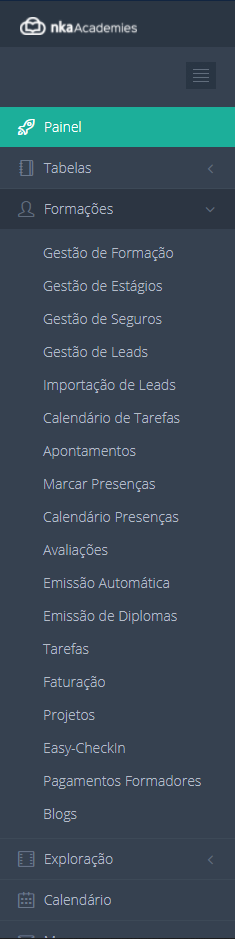
\includegraphics[width=\textwidth,height=0.5\textheight,keepaspectratio]{images/funcionalidades.png}
        \captionof{figure}{Gestão da formação}
        \label{fig:funcproduto}
\end{center}

O produto é ainda composto por uma plataforma para os seus \textbf{formadores} onde poderão encontrar entre outras, as seguintes funcionalidades (Figura~\ref{fig:professor}):
\begin{itemize}
  \setlength\itemsep{0em}
  \item Presenças e avaliações online
  \item Listagem detalhada da turma
  \item Sistema interno de mensagens
  \item Partilhar apontamentos e exercícios
  \item Informação na "cloud" sincronizada
  \item Histórico de formações
\end{itemize}

\begin{center}
        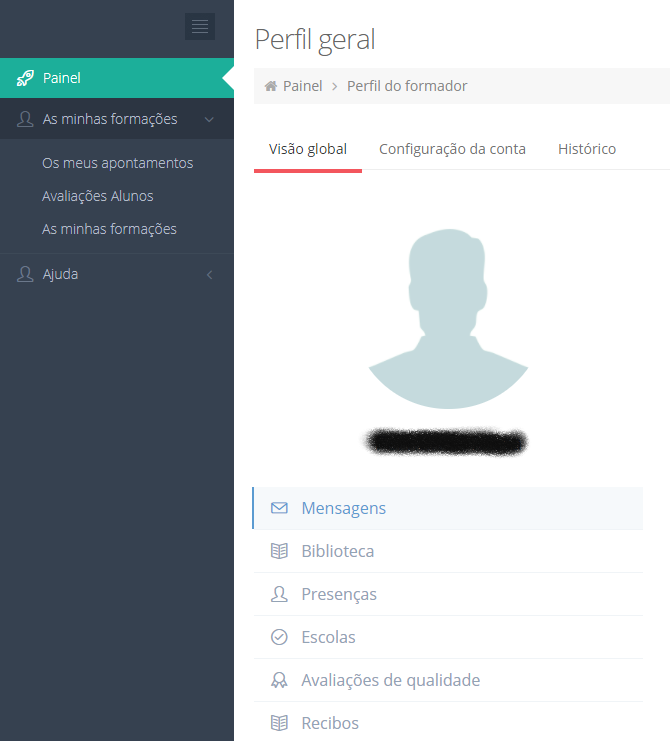
\includegraphics[width=\textwidth,height=\textheight,keepaspectratio]{images/professor.png}
        \captionof{figure}{Painel formador/professor}
        \label{fig:professor}
\end{center}

A plataforma disponibiliza também para os seus \textbf{alunos} e formandos um local onde poderão encontrar entre outras, as seguintes funcionalidades:
\begin{itemize}
  \item Partilha de diploma
  \item Descarregar manuais e documentos
  \item Devolver feedback
  \item Histórico de formação
  \item Manter o contacto com antigos colegas de formação
  \item Detalhes da formação
\end{itemize}

%---------------------
\section{Identificação das melhorias a realizar}

Atualmente, no mundo em que vivemos, \textit{updates} tecnológicos são lançados praticamente todos os dias relativos a sistemas de informação. É do maior interesse da parte de uma empresa, manter o seu produto atual e competitivo.

De momento, o produto NkaAcademies encontra-se desatualizado, utilizando versões antigas de \acrshort{php}(5.6) e MySQL. Foi então proposto desenvolver a migração de todo o produto NkaAcademies para as versões mais recentes do \acrshort{php}(5.6 -> 8.0.2) e do MySQL com o objetivo de atualizar o produto e também, de desenvolver novas funcionalidades que surgiram apenas em versões superiores à que o produto estava desenvolvido.

As melhorias a realizar passaram maioritariamente pela substituição total da biblioteca \acrshort{php} MySQL para MySQLi, uma vez que grande parte das funções que fazem parte da biblioteca MySQL foram descontinuadas, enquanto noutros casos apenas foram feitas alterações ao nível da chamada da função ou dos parâmetros (e ordem) recebidos. Posto isto, procedeu-se à sua alteração total no produto NkaAcademies, sendo que no caso de funções \textit{deprecated} foram implementadas alternativas \textit{hard-code} em \acrshort{php}.

Uma vez que se trata de uma migração completa de um produto pré-existente, o objetivo principal definido para o cumprimento desta fase tem a ver com a compatibilidade das alterações feitas. As novas funções e todas as modificações realizadas ao nível do produto devem ser implementadas tendo em vista a sua compatibilidade com as versões anteriores, que neste caso são as versões \acrshort{php} 5.6 e 7 e a compatibilidade com outras funcionalidades já existentes no produto garantindo a operabilidade e o bom funcionamento da aplicação na nova versão tecnológica.
%%--

\section{Alterações no desenvolvimento da solução}

Neste capítulo serão apresentadas algumas das principais alterações implementadas no produto NkaAcademies na fase da migração da aplicação para as versões mais recentes do \acrshort{php} e MySQL.

As principais alterações efetuadas no projecto NkaAcademies foram ao nível da chamadas de funções, implementação de novos métodos devido à descontinuidade de funções da biblioteca MySQL, parâmetros (e ordem) recebidos por funções e correções de erros de compatibilidade entre versões.

\subsection{Comparação de funções}

Neste sub-capítulo serão comparadas as funções das bibliotecas MySQL e MySQLi, em relação a \textit{inputs} e \textit{outputs} de algumas das funções utilizadas.

\subsubsection{\textit{mysql\_select\_db vs mysqli\_select\_db}}

Neste caso, será apresentado um excerto de código relativo a uma função que foi atualizada na biblioteca MySQLi, recebendo o mesmo tipo de parâmetros mas que trocou a ordem de como eram incorporados na função.

A função \textit{mysql\_select\_db} (listagem~\ref{lst:6}) seleciona uma base de dados do tipo MySQL.

\begin{lstlisting}[language={php},
                   caption={Função mysql\_select\_db.},
                   label=lst:6]
function mysql_select_db($database, $link_identifier=NULL):bool

\end{lstlisting}

A função da Listagem~\ref{lst:6} recebe como argumentos:
\begin{itemize}
  \item \textbf{\$database}: nome da base de dados que deverá ser selecionada.
  \item \textbf{\$link\_identifier}: conexão ao MySQL.
\end{itemize}


A função \textit{mysqli\_select\_db} (listagem~\ref{lst:7}) seleciona a base de dados a ser utilizada ao realizar \textit{queries} do tipo MySQLi.

\begin{lstlisting}[language={php},
                   caption={Função mysqli\_select\_db.},
                   label=lst:7]
    	function mysqli_select_db($mysql, $database):bool

\end{lstlisting}

A função da Listagem~\ref{lst:7} recebe como parâmetros:
\begin{itemize}
  \item \textbf{\$mysql}: \textit{connection string} de acesso à base de dados.
  \item \textbf{\$database}: nome da base de dados que deverá ser selecionada.
\end{itemize}

%-----

\subsubsection{\textit{mysql\_result vs nka\_mysqli\_result}}

Neste exemplo será apresentado nos excertos de código a alteração que teve de ser feita quando a função da biblioteca MySQL não foi continuada na biblioteca MySQLi, fazendo com que tivesse de ser criada uma equivalente.

A função \textit{mysql\_result} (listagem~\ref{lst:4}) obtém os dados de um determinado resultado.

\begin{lstlisting}[language={php},
                   caption={Função mysql\_result.},
                   label=lst:4]
    	function mysql_result($result, $row, $field=0):string

\end{lstlisting}

A função da Listagem~\ref{lst:4} recebe como argumentos:
\begin{itemize}
  \item \textbf{\$result}: resultado da \textit{query} \acrshort{sql} a ser executado.
  \item \textbf{\$row}: número da linha do resultado.
  \item \textbf{\$field}: nome do campo a ser procurado (tabela).
\end{itemize}


A função \textit{nka\_mysqli\_result} (listagem~\ref{lst:1}), utilizada para substituir a função \textit{deprecated mysql\_result} foi implementada recebendo os mesmos argumentos que a anterior, e retornando uma \textit{string}.\newpage

\begin{lstlisting}[language={php},
                   caption={Função para substituir mysql\_result.},
                   label=lst:1]
      if (!function_exists('nka_mysqli_result')) {
      	function nka_mysqli_result($res, $row, $field=0) {
      	  $res->data_seek($row);
      	  $datarow = $res->fetch_array();
      	  return $datarow[$field];
      	}
      }
\end{lstlisting}

A função da Listagem~\ref{lst:1} recebe como argumentos:
\begin{itemize}
  \item \textbf{\$result}: resultado da \textit{query} \acrshort{sql} a ser executado.
  \item \textbf{\$row}: número da linha do resultado.
  \item \textbf{\$field}: nome do campo a ser procurado (tabela).
\end{itemize}


\subsubsection{\textit{mysql\_field\_name vs mysqli\_field\_name}}

Nas Listagens~\ref{lst:5} e \ref{lst:2} está mais uma vez demonstrado o caso em que uma função da biblioteca MySQL é descontinuada para MySQLi e teve de se proceder à sua implementação.

A função \textit{mysql\_field\_name} (listagem~\ref{lst:5}) obtém o nome do campo especificado num resultado.


\begin{lstlisting}[language={php},
                   caption={Função mysql\_field\_name.},
                   label=lst:5]
  function mysql_field_name($result, $field_offset):string|false

\end{lstlisting}

A função da Listagem~\ref{lst:5} recebe como parâmetros:
\begin{itemize}
  \item \textbf{\$result}: resultado da \textit{query} \acrshort{sql} a ser executada.
  \item \textbf{\$field\_offset}: index/\textit{offset} de um campo numérico.
\end{itemize}


A função \textit{mysqli\_field\_name} (listagem~\ref{lst:2}), utilizada para substituir a função \textit{deprecated mysql\_field\_name} foi implementada no projeto recebendo os mesmos parâmetros que a anterior, e retornando uma \textit{string} ou \textit{false}.

\begin{lstlisting}[language={php},
                   caption={Função para substituir mysql\_field\_name.},
                   label=lst:2]
  if (!function_exists('mysqli_field_name')) {
    function mysqli_field_name($result, $field_offset){
$properties = mysqli_fetch_field_direct($result, $field_offset);
  return is_object($properties) ? $properties->name : false;
  }
  }
\end{lstlisting}

A função da Listagem~\ref{lst:2} recebe como parâmetros:
\begin{itemize}
  \item \textbf{\$result}: resultado da \textit{query} \acrshort{sql} a ser executada.
  \item \textbf{\$field\_offset}: index/\textit{offset} de um campo numérico.
\end{itemize}

%--

\subsection{Melhoria da função \textit{nka\_mysqli\_result}}

Neste caso está demonstrado um exemplo de uma melhoria de uma função que já tinha sido desenvolvida para substituir uma função descontinuada da biblioteca MySQL.

A função \textit{nka\_mysqli\_result\_v2} (listagem~\ref{lst:3}), foi um \textit{improvement} da função previamente implementada \textit{nka\_mysqli\_result}. Esta alteração deveu-se ao facto de alguns erros na incompatibilidade das diferentes versões(7 e 8) do \acrshort{php} em que o \textit{\$datarow} chegava \textit{empty}, enquanto que na versão \acrshort{php}5.6 a mesma função não apresentava erro. Verificou-se que a mesma função se comportava de forma diferente de versão para versão e como tal, procedeu-se à sua remodelação passando agora a retornar \textit{string} ou \textit{null} resolvendo o problema.


\begin{lstlisting}[language={php},
                   caption={Melhoria da função nka\_mysql\_result.},
                   label=lst:3]
      if (!function_exists('nka_mysqli_result_v2')) {
        function nka_mysqli_result_v2($res, $row, $field=0) {
      	  $res->data_seek($row);
      	  $datarow = $res->fetch_array();
      	  $retval = null;
      	  $cond = ! empty($datarow);
      	  if($cond){
      		    $retval = $datarow[$field];
      	  }
      	  return $retval;
      	}
      }
\end{lstlisting}

A função da Listagem~\ref{lst:3} recebe como argumentos:
\begin{itemize}
  \item \textbf{\$result}: resultado da \textit{query} \acrshort{sql} a ser executado.
  \item \textbf{\$row}: número da linha do resultado.
  \item \textbf{\$field}: nome do campo a ser procurado (tabela).
\end{itemize}

%\subsection{Paths}


% - falar que no 5.6 nka_mysqli_result nao acusava erro mas em versoes superiores 7 e 8 dava erro. A mesma funçao comportava-se diferente nas 2 versões desenvolvidas.
